\documentclass[12pt,a4paper]{report}
\usepackage[brazil]{babel}
\usepackage[]{algorithm}
\usepackage[]{algorithmic}

\usepackage[style=numeric,backend=biber]{biblatex}
\usepackage[utf8]{inputenc}
\usepackage{kpfonts}
\usepackage[T1]{fontenc}
\usepackage{wrapfig}
\usepackage{graphicx}
\usepackage{enumerate}
\usepackage{subcaption}
\usepackage{float}
\usepackage{caption}
\usepackage{listings}
\usepackage{lipsum}
\usepackage{amsthm}
\usepackage{amssymb}
\usepackage{bm}
\usepackage{color}
\usepackage{afterpage}
\usepackage[inline]{enumitem}
\usepackage{pdflscape}
\usepackage{listingsutf8}
\usepackage{siunitx}
\usepackage{bashful}

\usepackage{hyperref}
\hypersetup{
    colorlinks=true,
    linkcolor=blue,
    filecolor=magenta,      
    urlcolor=cyan,
}

\usepackage[margin=1in]{geometry}

\lstset{frame=tb,
  aboveskip=2mm,
  belowskip=2mm,
  showstringspaces=false,
  columns=flexible,
  basicstyle=\footnotesize,,
  numbers=left,
  numbersep=5pt,
  stepnumber=1,
  breaklines=true,
  keepspaces=true,
  breakatwhitespace=true,
  showtabs=false,  
  tabsize=2
}


% Definindo estilo para os códigos
\definecolor{mGreen}{rgb}{0,0.6,0}
\definecolor{mGray}{rgb}{0.5,0.5,0.5}
\definecolor{mPurple}{rgb}{0.58,0,0.82}
\definecolor{dkgreen}{rgb}{0,0.6,0}
\definecolor{backgroundColour}{rgb}{0.97,0.97,0.97}

\lstset{basicstyle=\ttfamily,
    backgroundcolor=\color{backgroundColour},   
    commentstyle=\color{mGreen},
    keywordstyle=\color{magenta},
    numberstyle=\tiny\color{mGray},
    commentstyle=\color{dkgreen},
    stringstyle=\color{mPurple},
    basicstyle=\footnotesize,
    breakatwhitespace=false\textbf{,}         
    breaklines=true,                 
    captionpos=b,                    
    keepspaces=true,                 
    numbers=left,                    
    numbersep=5pt,                  
    showspaces=false,                
    showstringspaces=false,
    showtabs=false,                  
    tabsize=2,
    language=bash
}

\lstdefinestyle{BStyle}{
    backgroundcolor=\color{backgroundColour},  
    showstringspaces=false,
    numbers=none,
    language=bash
}

\pagenumbering{arabic}
\renewcommand{\thesection}{\arabic{section}}

\bibliography{ref}
\renewcommand{\contentsname}{Sumário}{\thispagestyle{empty}}
\renewcommand{\baselinestretch}{1.5} 

\begin{document}

\begin{titlepage}
        \begin{center}
                \vspace*{1cm}
                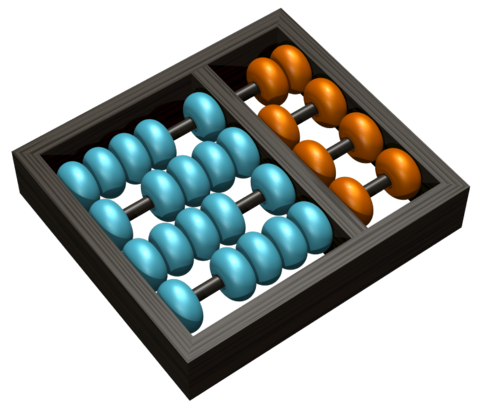
\includegraphics[width=0.25\textwidth]{Logo}\\
                \vspace{1.5cm}
                \Huge
                \textbf{Exercício 5}\\
                \vspace{1.5cm}
                \Large
                \textbf{Aluno}: João Vitor Gonçalves\\
                \textbf{RA}: 176353\\
                \vspace{1.2cm}
                \Large
                Instituto de Computação\\
                Universidade Estadual de Campinas\\
                \vspace{1.5cm}
                Campinas, 19 de Dezembro de 2020.
        \end{center}
\end{titlepage}
\tableofcontents
\clearpage

\newcommand{\shellcmd}[1]{\texttt{\footnotesize\# #1}}%estilizando citação de comandos do shell

\section{Funcionamento do exercício.}

O funcionamento do programa se dá da seguinte maneira:

Temos dois executáveis distintos, o servidor que pode ser executado da seguinte forma:

\begin{lstlisting}[language=bash]
    ./lab/build/server/server [PORT]
\end{lstlisting}


E o cliente:
\begin{lstlisting}[language=bash]
    ./lab/build/client/client [SERVER_IP] [PORT]
\end{lstlisting}

\bigbreak

É necessário ter o servidor sendo executado antes de iniciar o cliente.

\bigbreak

Ao iniciar o cliente, ele irá se conectar ao servidor, e irá pedir o input do identificador desejado.

\begin{figure}[H]
    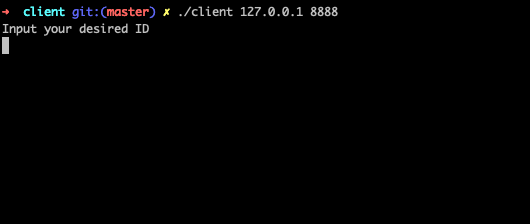
\includegraphics[width=\linewidth]{id_input.png}
    \caption{Cliente pedindo input de um ID.}
\end{figure}

O cliente irá pedir a confirmação da escolha. 

\begin{figure}[H]
    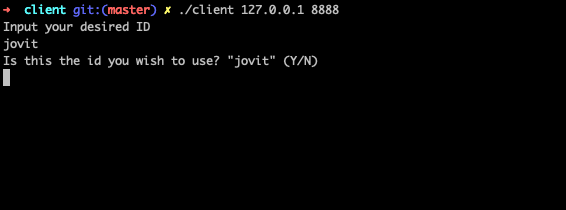
\includegraphics[width=\linewidth]{id_input_conf.png}
    \caption{Cliente confirmando escolha do ID.}
\end{figure}

Caso confirmado, o ID será enviado para o servidor. Que pode confirmar caso o ID esteja disponível, e negar caso já exista algum outro usuário utilizando o mesmo ID.

\begin{figure}[H]
    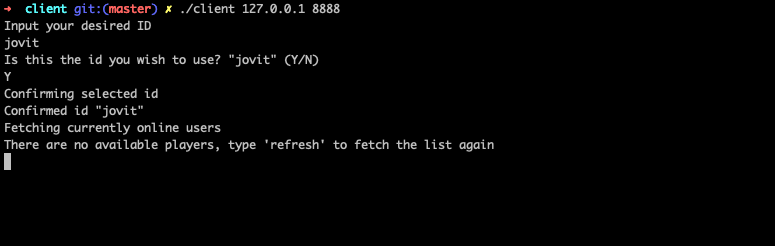
\includegraphics[width=\linewidth]{id_input_success.png}
    \caption{Seleção de ID confirmada com sucesso pelo servidor.}
\end{figure}

\begin{figure}[H]
    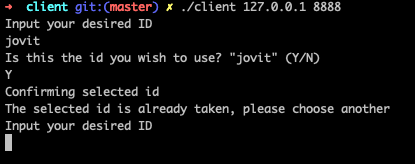
\includegraphics[width=\linewidth]{input_id_fail.png}
    \caption{Falha na seleção de ID.}
\end{figure}

No caso de falha, o cliente pede ao usuário para escolher um outro ID.

\bigbreak

Caso a seleção de um identificador seja bem sucedida. A lista de usuários disponíveis para um jogo será exibida.
\begin{figure}[H]
    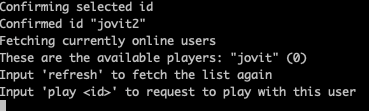
\includegraphics[width=\linewidth]{user_list.png}
    \caption{Listagem de usuários disponíveis para jogar.}
\end{figure}

O usuário poderá atualizar essa lista por meio do comando \emph{refresh} ou jogar com algum dos usuários disponíveis por meio do comando \emph{play <id>}. 

eg:
\begin{lstlisting}[language=bash]
    play jovit
\end{lstlisting}

\bigbreak

Caso enviado o comando de jogar, uma requisição será enviada para o cliente correspondente:

\begin{figure}[H]
    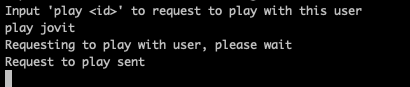
\includegraphics[width=\linewidth]{request_sent.png}
    \caption{Requisição de jogo enviada.}
\end{figure}

E o usuário requisitado irá receber uma notificação perguntando se ele deseja jogar:

\begin{figure}[H]
    
\includegraphics[width=\linewidth]{request_received.png}
    \caption{Requisição de jogo recebida.}
\end{figure}

\bigbreak

No caso de confirmação, ambos os clientes irão enviar as suas portas UDP para o servidor, que em seguida irá compartilhar o endereço IP e portas de cada um dos clientes para que eles possam se comunicar diretamente via datagramas UDP.

\begin{figure}[H]
    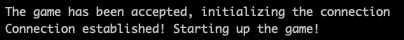
\includegraphics[width=\linewidth]{udp_connection.png}
    \caption{Teste de conexão é feito entre os clientes antes de iniciar o jogo.}
\end{figure}

\bigbreak

Então em seguinda, o jogo é iniciado:

\bigbreak

Primeiro, cada um dos clientes sorteia um número de 0 à 100, e o usuário com o maior número joga primeiro.

\begin{figure}[H]
    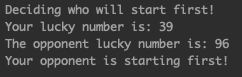
\includegraphics[width=\linewidth]{lucky_number.png}
    \caption{Sorteio de quem irá iniciar o jogo.}
\end{figure}

\bigbreak

Então é exibido o tabuleiro do jogo:

\begin{figure}[H]
    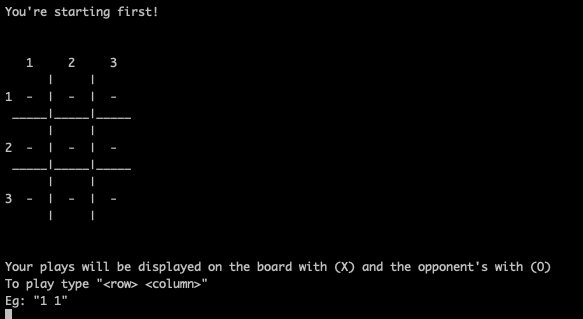
\includegraphics[width=\linewidth]{game_board.png}
    \caption{Tabuleiro do jogo.}
\end{figure}

As jogadas do usuário serão exibidas com o símbolo \textbf{X} e as do oponente com o símbolo \textbf{O}.

Jogadas são feitas escrevendo o número da linha seguido do número da coluna que se deseja jogar.

Após cada jogada, ela é transmitida para o oponente e é checado se o jogo está finalizado.

\begin{figure}[H]
    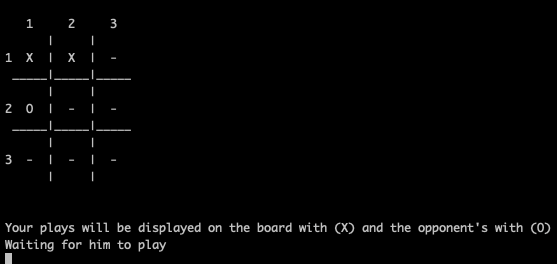
\includegraphics[width=\linewidth]{game.png}
    \caption{Tabuleiro do jogo.}
\end{figure}

\bigbreak

Ao final do jogo, é atribuído pontuações da seguinte maneira: No caso de vitória, o usuário ganha 1 ponto, no caso de perda ele perde 1 ponto (com pontuação mínima de 0), e no caso de empate ele não ganha nenhum ponto.

Cada um dos clientes transmite a sua pontuação para o servidor, que retorna a pontuação consolidada atual:

\begin{figure}[H]
    
\includegraphics[width=\linewidth]{points.png}
    \caption{Pontuação do usuário.}
\end{figure}

\bigbreak

Em sequência, a lista dos usuários disponíveis é exibida, para que o jogador possa iniciar uma nova partida:

\begin{figure}[H]
    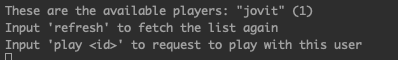
\includegraphics[width=\linewidth]{players.png}
    \caption{Jogadores.}
\end{figure}

Na lista de jogadores disponíveis, as suas pontuações são exibidas entre parênteses após seus IDs.

Por questões de simplificação de testes, o servidor só guarda a pontuação dos usuários conectados, caso um usuário se desconecte, a sua pontuação anterior é perdida. Porém as pontuações para cada identificador poderiam fácilmente ser guardadas em arquivos.

\bigbreak

Um caso de falha que não foi considerado no desenvolvimento, foi o caso de um cliente se desconectar durante uma partida. Nesse caso o seu oponente ficará aguardando uma jogada perpetuamente. Isso foi feito para simplificar a comunicação udp durante o jogo, que para tratar esse caso, deveria ser feita usando multiplexação de entrada e saída.

\section{Compilação}

Para realizar a compilação da aplicação, basta executar o script \emph{build.sh} fornecido.

\begin{lstlisting}[language=bash]
    cd ./lab
    ./build.sh
\end{lstlisting}

\end{document}